\section{Idé}

\begin{frame}{Hvad er problemet?}
Reducere brændsstofforbug
\begin{itemize}
\item Miljøhensyn
\item Økonomihensyn
\end{itemize}

Muligheder
\begin{itemize}
\item Mindre skadelig eller ny type brændstof
\item \textbf{Brændstofbesparende kørsel}
\item ...
\end{itemize}
\end{frame}

\begin{frame}{Brændstofbesparende kørsel}
Muligheder
\begin{itemize}
\item Korrekt gearskifte
\item \textbf{Minimere acceleration}
\item ...
\end{itemize}

Forhindinger
\begin{itemize}
\item Anden trafik
\item \textbf{Trafiklys}
\item ...
\end{itemize}

\end{frame}

\begin{frame}{Trafiklys}
Muligheder
\begin{itemize}
\item Adaptive trafiklys
\item \textbf{Tilpasse bilers hastighed til trafiklysene}
\item ...
\end{itemize}


\begin{center}
\begin{columns}
\begin{column}{0.5\textwidth}
Fordele
\begin{itemize}
\item Ingen ekstra udstyr, dog forbindelse til biler - evt. centralt
\item Få opstartsudgifter 
\item Virker ved lav penetrationsrate
\end{itemize}
\end{column}

\begin{column}{0.5\textwidth}
Ulemper
\begin{itemize}
\item Kræver biler kan aflæse trafiksignaler
\item Påvirkning af øvrig trafik?
\end{itemize}
\vspace{1.2cm}
\end{column}
\end{columns}
\end{center}
\end{frame}

\begin{frame}{Idé}
\begin{center}
Kan man med \textbf{information} om trafiksignaler og evt. trængsel\\\textbf{spare brændstof} for den enkelte bil\\uden påvirkning af anden trafik?
\end{center}
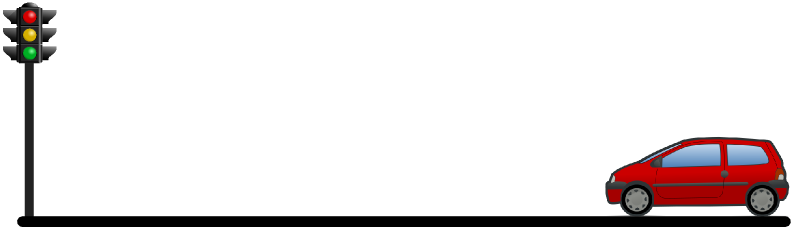
\includegraphics[width=1\textwidth]{images/figure.png}
\end{frame}

\begin{frame}{Hastighedstilpasning}
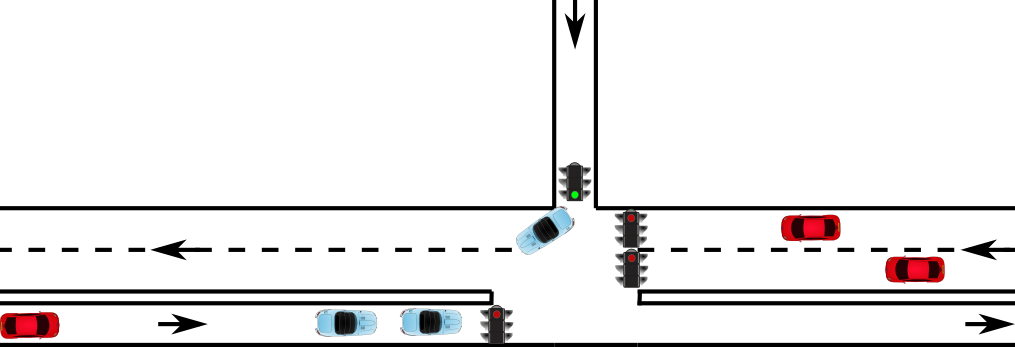
\includegraphics[width=1\textwidth]{images/eks1.png}
\end{frame}

\begin{frame}{Hastighedstilpasning}
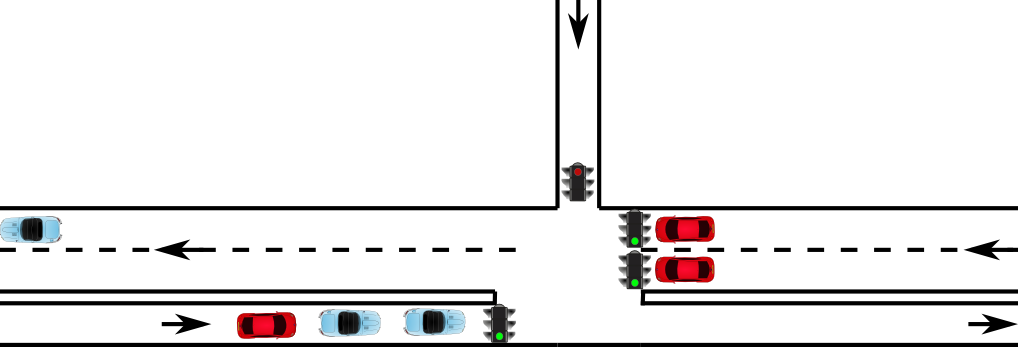
\includegraphics[width=1\textwidth]{images/eks2.png}
\end{frame}

